\documentclass[12pt,a4paper]{report}
\usepackage[a4paper,margin=1in]{geometry}
\usepackage{graphicx}
\usepackage{lmodern}
\usepackage{setspace}
\usepackage{titlesec}
\usepackage{lipsum}
\usepackage{fancyhdr}
\usepackage{xcolor}
\usepackage{float}
\usepackage[Sonny]{fncychap}

\newcommand{\todo}[1]{\fcolorbox{black}{yellow}{\textbf{TODO:} #1}}

%--------------------------------
% Chapter Title
%--------------------------------
\ChNameVar{\raggedleft\bfseries\Large}   % "CHAPTER" word
\ChNumVar{\raggedleft\bfseries\Large}    % Chapter number
\ChTitleVar{\raggedleft\bfseries\Large}  % Chapter title

%--------------------------------
% Section Title
%--------------------------------
\titleformat{\section}[block]
    {\titlerule[2pt]\addvspace{0.8ex}%
    \bfseries\Large}
    {\thesection}{0.5em}
    {}[{\addvspace{0.4ex}\titlerule[2pt]}]
\titlespacing{\section}{0pt}{*4}{*4}

% Display current section in header:
\pagestyle{fancy}
\fancyhf{}
\fancyhead[L]{\nouppercase{\rightmark}}
\fancyfoot[C]{\thepage}

\begin{document}

% Title Page
\begin{titlepage}
    \centering
    
    % University logo at the top
    
\includegraphics[width=0.3\textwidth]{images/uantwerp_logo.png}\\[1cm]
    
    {\Huge \textbf{Multimodal Data Integration for Predictive Modelling of Measles Vaccine Response with Cross-Vaccine Marker Validation}} \\
    \vfill
    
    {\Large \textbf{Elias Dams}}\\[1cm]
    
    \textbf{Promotor:} Dr. Pieter Meysman\\
    \textbf{Supervisor:} Fabio Affaticati\\[1.5cm]
    
    {\Large \textbf{University of Antwerp}}\\
    {\large Faculty of Science}\\[0.5cm]
    
    \textbf{2024-2025}\\[1.5cm]
    
    Submitted in fulfilment of the requirements for the degree of\\
    \textbf{Master in Computer Science: AI \& Data Science}\\[1cm]
    
    \textbf{June 2025}\\[2cm]
    
    % Decorative line at the bottom
    \vfill
    
\includegraphics[width=1.0\textwidth]{images/bottom_design.jpg}

\end{titlepage}

% Table of Contents
\tableofcontents
\newpage

% List of Figures, Tables, Acronyms
\listoffigures

\listoftables

\chapter*{List of Acronyms}
- TCR: T-cell receptor

% Preliminary Sections
\chapter*{Summary}

\chapter*{Acknowledgements}

\chapter*{Abstract}


% Chapters
\chapter{Introduction}
Vaccination is one of the most cost-effective strategies to prevent infectious diseases; however, individuals often exhibit very different responses to the same vaccine. This thesis focuses on predicting responses to the measles vaccine using a data-driven, multimodal approach. The ultimate goal is to develop predictive models that not only forecast individual vaccine responses but also validate key immune markers across different vaccines. This process is known as cross-vaccine marker validation.\\
\\
From a computer science perspective, my work leverages machine learning techniques to integrate diverse types of biological data. In this study, I combine measurements of immune system responses, such as cytokine levels and cell counts obtained from cytometry, with molecular profiling data, including antibody titers and T cell receptor (TCR) sequences. For instance, antibody titers, which quantify the concentration of specific antibodies in the blood, serve as a direct indicator of the immune system’s ability to neutralise pathogens. Cytokine levels provide early signals about the body’s readiness to respond, while TCR sequencing reveals which T cell clones are active and specific to the vaccine antigen.\\
\\
Initially, I work with measles data from a study comprising 40 samples. While this dataset provides a valuable starting point, its relatively small size poses challenges in terms of statistical power and model generalisability. Furthermore, integrating heterogeneous data types introduces additional difficulties, such as differing scales, potential noise, and missing values, all of which must be carefully addressed during data preprocessing and feature selection.\\
\\
\todo{info about the study my data is coming from.}\\
\\
In the following chapters, I will detail the processes of data exploration, feature selection, model building, and validation that underpin this multimodal approach. This work aims not only to improve our ability to predict vaccine responses but also to enhance our understanding of the immune markers that are most relevant for effective immunisation across different vaccines.

\chapter{Background}

To understand the work presented in this thesis, it is essential to have a basic grasp of concepts from both immunology and data science. As a computer scientist, my approach is mainly data-driven, focusing on extracting, integrating, and analysing various types of biological data. However, a foundational understanding of the underlying biological processes is critical to meaningfully interpret the results and validate the predictive models developed in this research.

\section{Background in Biology}

\subsection{Immune System Overview}

\begin{figure}[h]
  \centering
  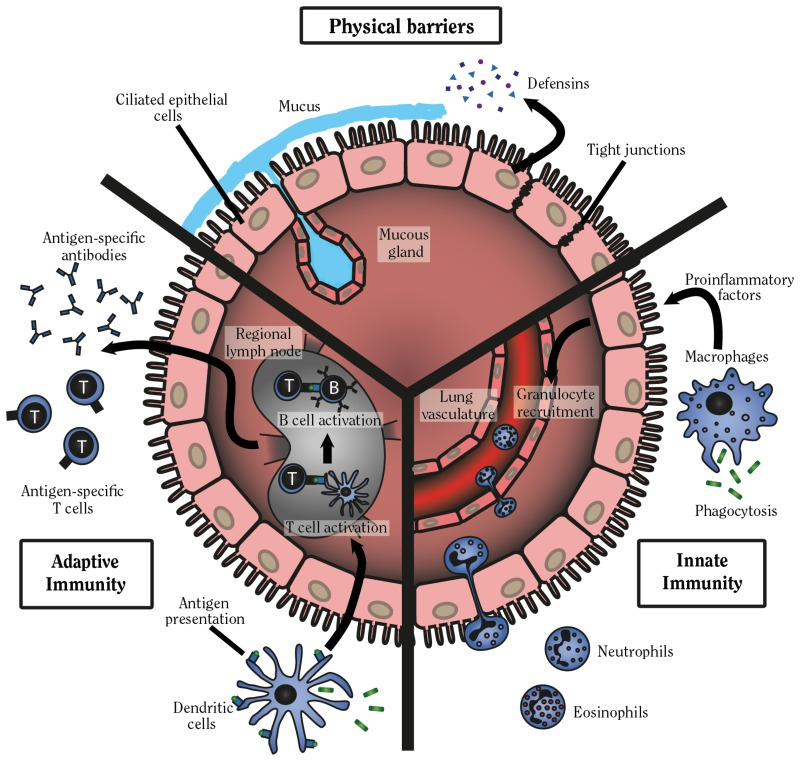
\includegraphics[width=0.8\textwidth]{images/Diagram_of_innate_and_adaptive_immunity.jpg}
  \caption[Diagram of Innate and Adaptive Immunity]{Diagram showing physical barriers, innate immune cells (e.g., macrophages, dendritic cells, natural killer cells) and adaptive immune components (B and T cells) working together. Reproduced from Figure 10.5 in \emph{The Health Consequences of Smoking—50 Years of Progress: A Report of the Surgeon General} (2014) \cite{smoking2014}.}
  \label{fig:immunity}
\end{figure}

First of all, I would like to give an overview of how the immune system works. The immune system can be roughly divided into three main parts, as depicted in Figure \ref{fig:immunity}:\\
\\
\textbf{Physical barriers (top)}\\
Physical barriers such as the skin and mucous membranes form the body’s first line of defence by preventing most pathogens from entering.\\
\\
\textbf{Innate Immunity (right)}\\
In case a pathogen still crosses the barriers, innate immunity comes into action. This defence is rapid and non-specific. Think of macrophages and neutrophils as cells that engulf invaders through a process called phagocytosis. Eosinophils and other granulocytes also attack pathogens or initiate inflammatory responses. Natural killer cells (NK cells) are also part of innate immunity and can directly destroy infected or abnormal cells. Although this response is very rapid, it does not recognise pathogens in the same specific way as the next branch. \cite{janeway2001immunobiology}\\
\\
\textbf{Adaptive Immunity (left)}\\
Acquired or adaptive immunity is the “slower but more targeted” defence. B cells are an important part here. They are responsible for producing antibodies, which are proteins that bind to specific antigens (foreign substances) to neutralise or mark them for destruction. The level of these antibodies in the blood is often measured as “antibody titers". Higher titers generally indicate a stronger immune response. T cells are also crucial and have several roles. They help coordinate the immune response (often referred to as “helper T cells”) and can directly kill infected cells (cytotoxic T cells). T cell receptors (TCRs) are highly specific and can be sequenced to understand which T cell clones are active in response to a vaccine. A major advantage of adaptive immunity is that it “learns” from previous exposure, allowing for much faster and more powerful immune responses in the event of repeated infection. This ability to form memory also underlies how vaccines work. \cite{janeway2001immunobiology}\\
\\
Together, these three pillars provide a robust defence system that is able to successfully ward off or fight off most infections. It is also this dynamic between innate and adaptive immunity that determines the degree of vaccine response. the innate branch prepares the way, while the adaptive branch provides targeted antibodies and memory cells. This is important to understand because my models integrate elements of both the innate and adaptive immune systems. For example, innate markers such as cytokine levels and certain cell counts (measured via cytometry) can provide early signals about the body's general readiness to respond. Meanwhile, adaptive markers, such as TCR sequences of T cells, directly reflect the specific immune response that leads to antibody production after vaccination. Combining this data gives us a more complete picture of the immune landscape, allowing me to better predict how effectively an individual will respond to the measles vaccine.

\subsection{Antibody Titers }
In addition to assessing the cellular components of the immune response, it is crucial to quantify the functional output of the adaptive immune system, namely antibody production. Antibody titers provide a quantitative measurement of the concentration of specific antibodies in the blood, and essentially reflect the “signal strength” of the immune response against a particular antigen. High titers usually mean that the immune system is actively fighting off the pathogen by targeting and clearing it effectively. In contrast, low titers indicate a weaker response and thus less robust protection.\\
\\
To determine antibody titers in the laboratory, serial dilution tests are often used. In these tests, a serum sample is progressively diluted and each dilution tests its ability to bind to the target antigen. The titer is defined as the highest dilution at which antibodies can still be detected. This method allows a practical estimate of the antibody concentration in the original sample.\\
\\
In my research thesis, antibody titers serve as an important biomarker to label vaccine response categories. By categorising individuals based on their antibody titers, I can distinguish between strong and weak responders. This classification is essential for developing and validating predictive models because it provides a clear, quantifiable endpoint that reflects the effectiveness of the measles vaccine in eliciting a protective immune response.

\pagebreak
\section{Background in Computer science}
\todo{info about the used computer science techniques.}\\

\pagebreak
\chapter{Data Exploration and Preprocessing}
In this chapter, I describe how the measles antibody titer data was prepared and how response labels were assigned. 
\todo{...}\\

\section{Label Assignment Strategy}
\noindent
The original dataset included antibody titer measurements at four time points (Day0, Day21, Day150, and Day365), as well as detailed qualitative classifications for each subject (e.g. \texttt{responder},  \texttt{no response - high ab} and \texttt{no response - low ab}). However, these classifications were too specific for the initial stages of modeling. Consequently, I reduced the labels to a simple, two-class scheme (e.g. \texttt{responder} and \texttt{non-responder}) to create a more straightforward prediction task that can be refined later if necessary. 

\section{Antibody Titer Trajectories}

\subsection{By Response Label}
\noindent
Figure~\ref{fig:titer_response_label} shows the antibody titer trajectories over four time points, separated by each subject’s final response label (\texttt{response} or \texttt{no response}). On the x-axis, we have the days at which titers were measured (0, 21, 150, 365). The y-axis represents the titer level. Each line corresponds to a single subject’s progression across these time points. From this visualization, it is evident that “responders” generally exhibit a marked increase in titers between Day 0 and Day 21 (and sometimes up to Day 150), whereas “non-responders” show either a small rise or a plateau. This distinction validates the simplified two-class approach used for model building. In contrast, Figure~\ref{fig:titer_original_label} displays the antibody titer trajectories based on the original, more granular labels (i.e., \texttt{responder}, \texttt{no response - high ab}, and \texttt{no response - low ab}). 

\begin{figure}[H]
\centering
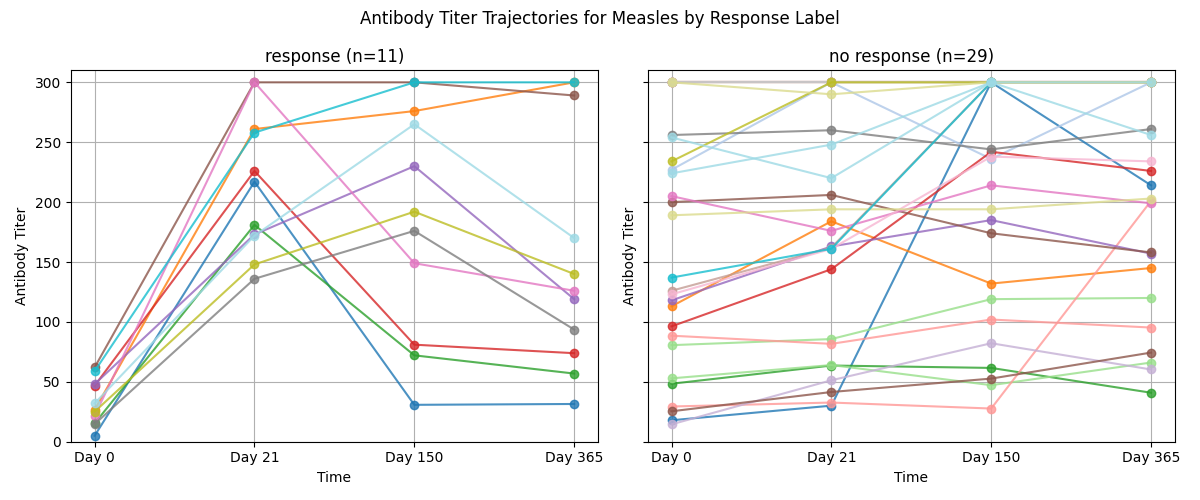
\includegraphics[width=0.9\textwidth]{images/Antibody_Titer_Trajectories_for_Measles_by_Response_Label.png}
\caption[Antibody Titer Trajectories by Response Label]{Antibody titer trajectories for each subject, colored by final response label. Subjects labeled as \texttt{response} are shown in green, while those labeled as \texttt{no response} are shown in orange.}
\label{fig:titer_response_label}
\end{figure}

\begin{figure}[H]
\centering
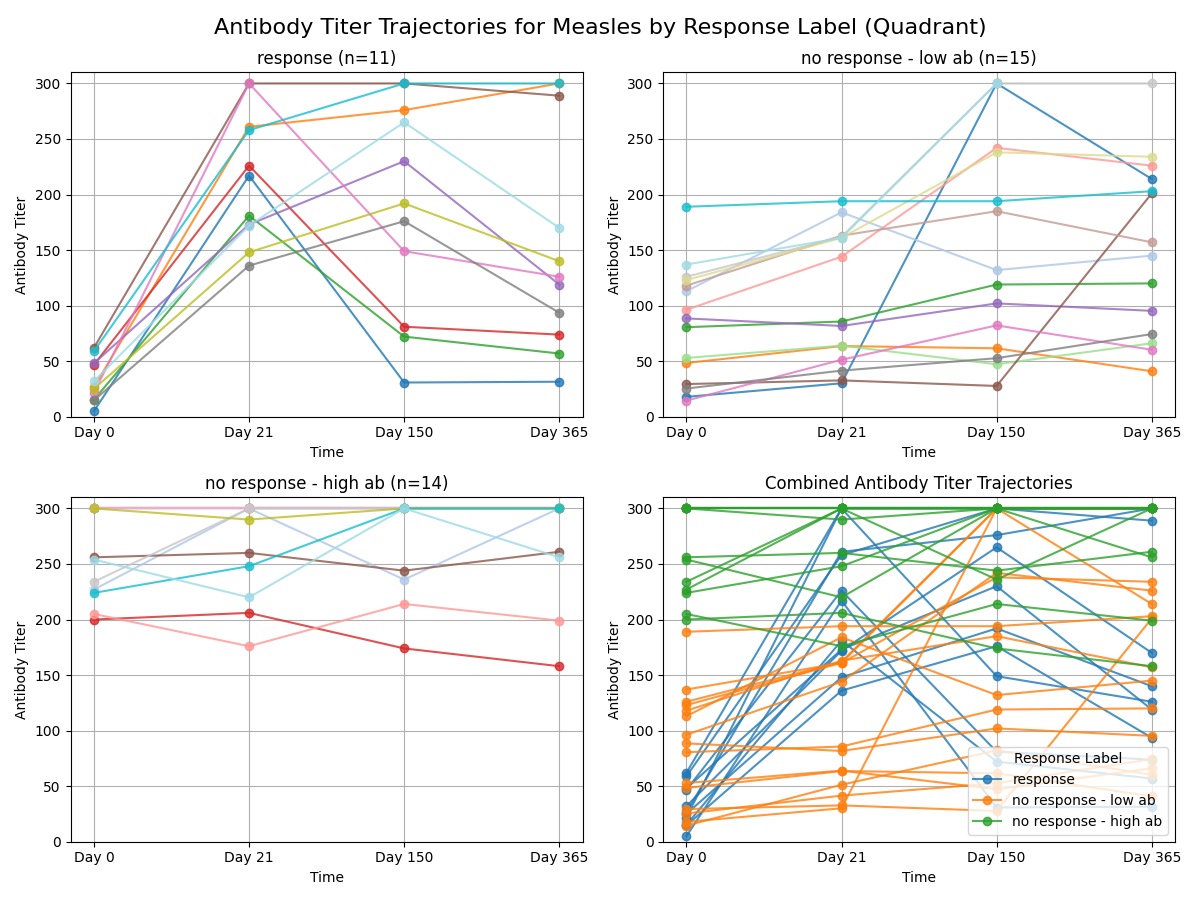
\includegraphics[width=0.9\textwidth]{images/Antibody_Titer_Trajectories_for_Measles_by_Original_Label_(Quadrant).png}
\caption[Antibody Titer Trajectories by Original Label (Quadrant)]{Antibody titer trajectories for each subject, colored by the original qualitative labels (quadrant). This view highlights the detailed categorization of responses, offering insights into the nuances of each subject’s titer progression.}
\label{fig:titer_original_label}
\end{figure}

\pagebreak
\noindent
The simplified \texttt{response\_label} variable is used throughout the thesis as the target for classification tasks. This choice reduces complexity, addressing both data imbalance and interpretability concerns. While the dataset initially contained more nuanced labels (e.g., distinguishing “no response - high ab” from “no response - low ab”), combining them into a single “no response” category improves the feasibility of training robust machine learning models given the limited sample size.\\

\section{Correlation Analysis Within Individual Datasets}
\noindent
In this chapter, I explore the interrelationships among the variables in the different datasets. The data consist of five distinct datasets:
\begin{itemize}
\item Cytokines
\item Cytometry
\item clonal  breadth (TCR metrics )
\item clonal depth (TCR metrics )
\item RNA data
\end{itemize}
Because each dataset captures different aspects of the immune response, I begin by investigating correlations within each individual dataset. Subsequently, I concatenate the datasets to perform an integrated correlation analysis. This approach allows me to uncover both within-modality and cross-modality relationships.
\subsection{Methodology}
\noindent
\todo{Check if right...}
In my analysis, I use a Weighted Gene Co-expression Network Analysis (WGCNA) framework to identify modules of highly correlated features. First, I compute a correlation matrix from the data, which quantifies the pairwise relationships between features. This correlation matrix is then transformed into a distance matrix by taking one minus the absolute correlation value, ensuring that strongly correlated features are considered close. Instead of relying on a fixed linkage method like Ward.D2, WGCNA integrates hierarchical clustering with network analysis to detect modules, or clusters, of co-expressed features. In the implementation, I use the \texttt{flashClust} package for efficient hierarchical clustering, and then apply a dynamic tree cut procedure to define the modules. The modules are further visualized by assigning each a unique color using WGCNA’s labeling functions and displaying the resulting dendrogram and heatmap plots. This approach captures complex correlation patterns, effectively groups similar features. Moreover, by merging datasets from different modalities, we can explore both within-modality and cross-modality relationships, ultimately facilitating more effective downstream machine learning tasks.

\pagebreak
\subsection{Cytokine Data}
\begin{figure}[H]
  \centering
  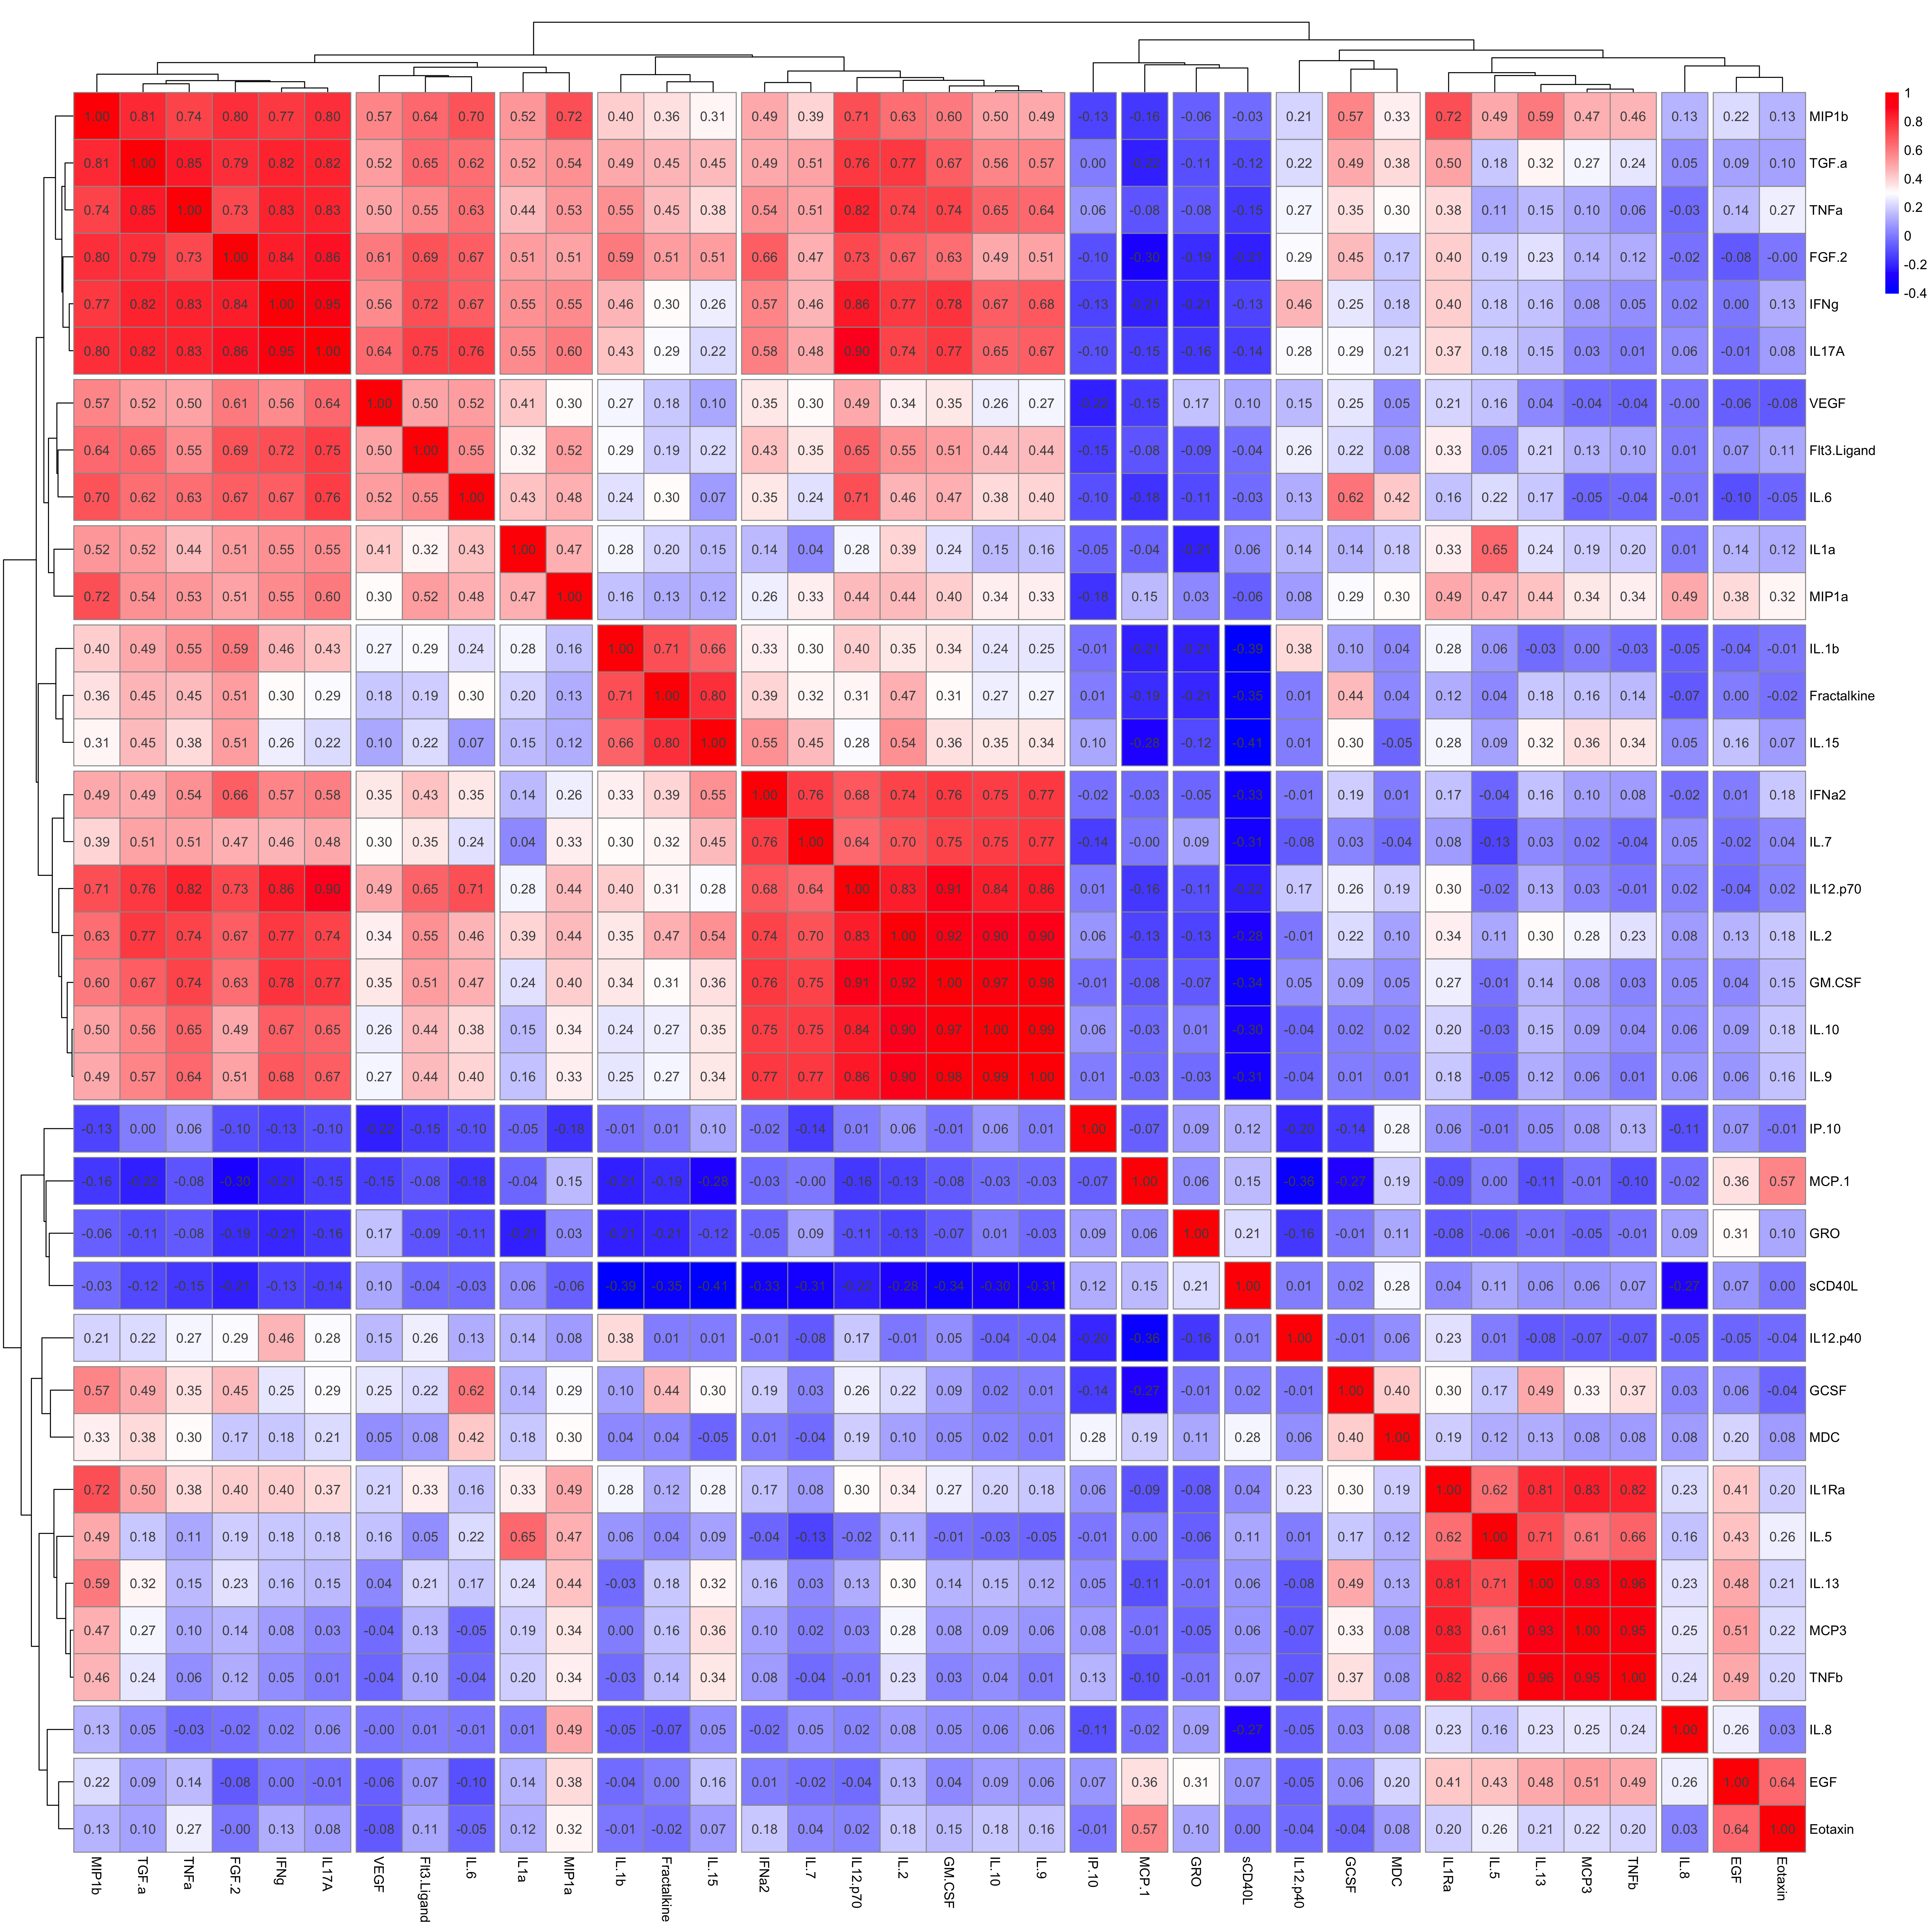
\includegraphics[width=0.8\textwidth]{images/Cytokine_euclidean_distance.png}
  \caption{Correlation heatmap of the cytokine data using Ward.D2 clustering.}
  \label{fig:cytokine_heatmap}
\end{figure}

The following cytokine clusters were obtained from the WGCNA hierarchical clustering analysis:

\begin{itemize}
    \item \textbf{Cluster 1:} MIP1$\beta$, TGF-$\alpha$, TNF-$\alpha$, FGF-2, IFN-$\gamma$, IL17A.
    \item \textbf{Cluster 2:} VEGF, Flt3 Ligand, IL-6.
    \item \textbf{Cluster 3:} IL1$\alpha$, MIP1$\alpha$.
    \item \textbf{Cluster 4:} IL-1$\beta$, Fractalkine, IL-15.
    \item \textbf{Cluster 5:} IFN$\alpha$2, IL-7, IL12-p70, IL-2, GM-CSF, IL-10, IL-9.
    \item \textbf{Cluster 6:} IL1Ra, IL-5, IL-13, MCP3, TNF$\beta$.
    \item \textbf{Cluster 7:} GCSF, MDC.
    \item \textbf{Cluster 8:} EGF, Eotaxin.
\end{itemize}

\subsection{Cytometry Data}

\begin{figure}[H]
  \centering
  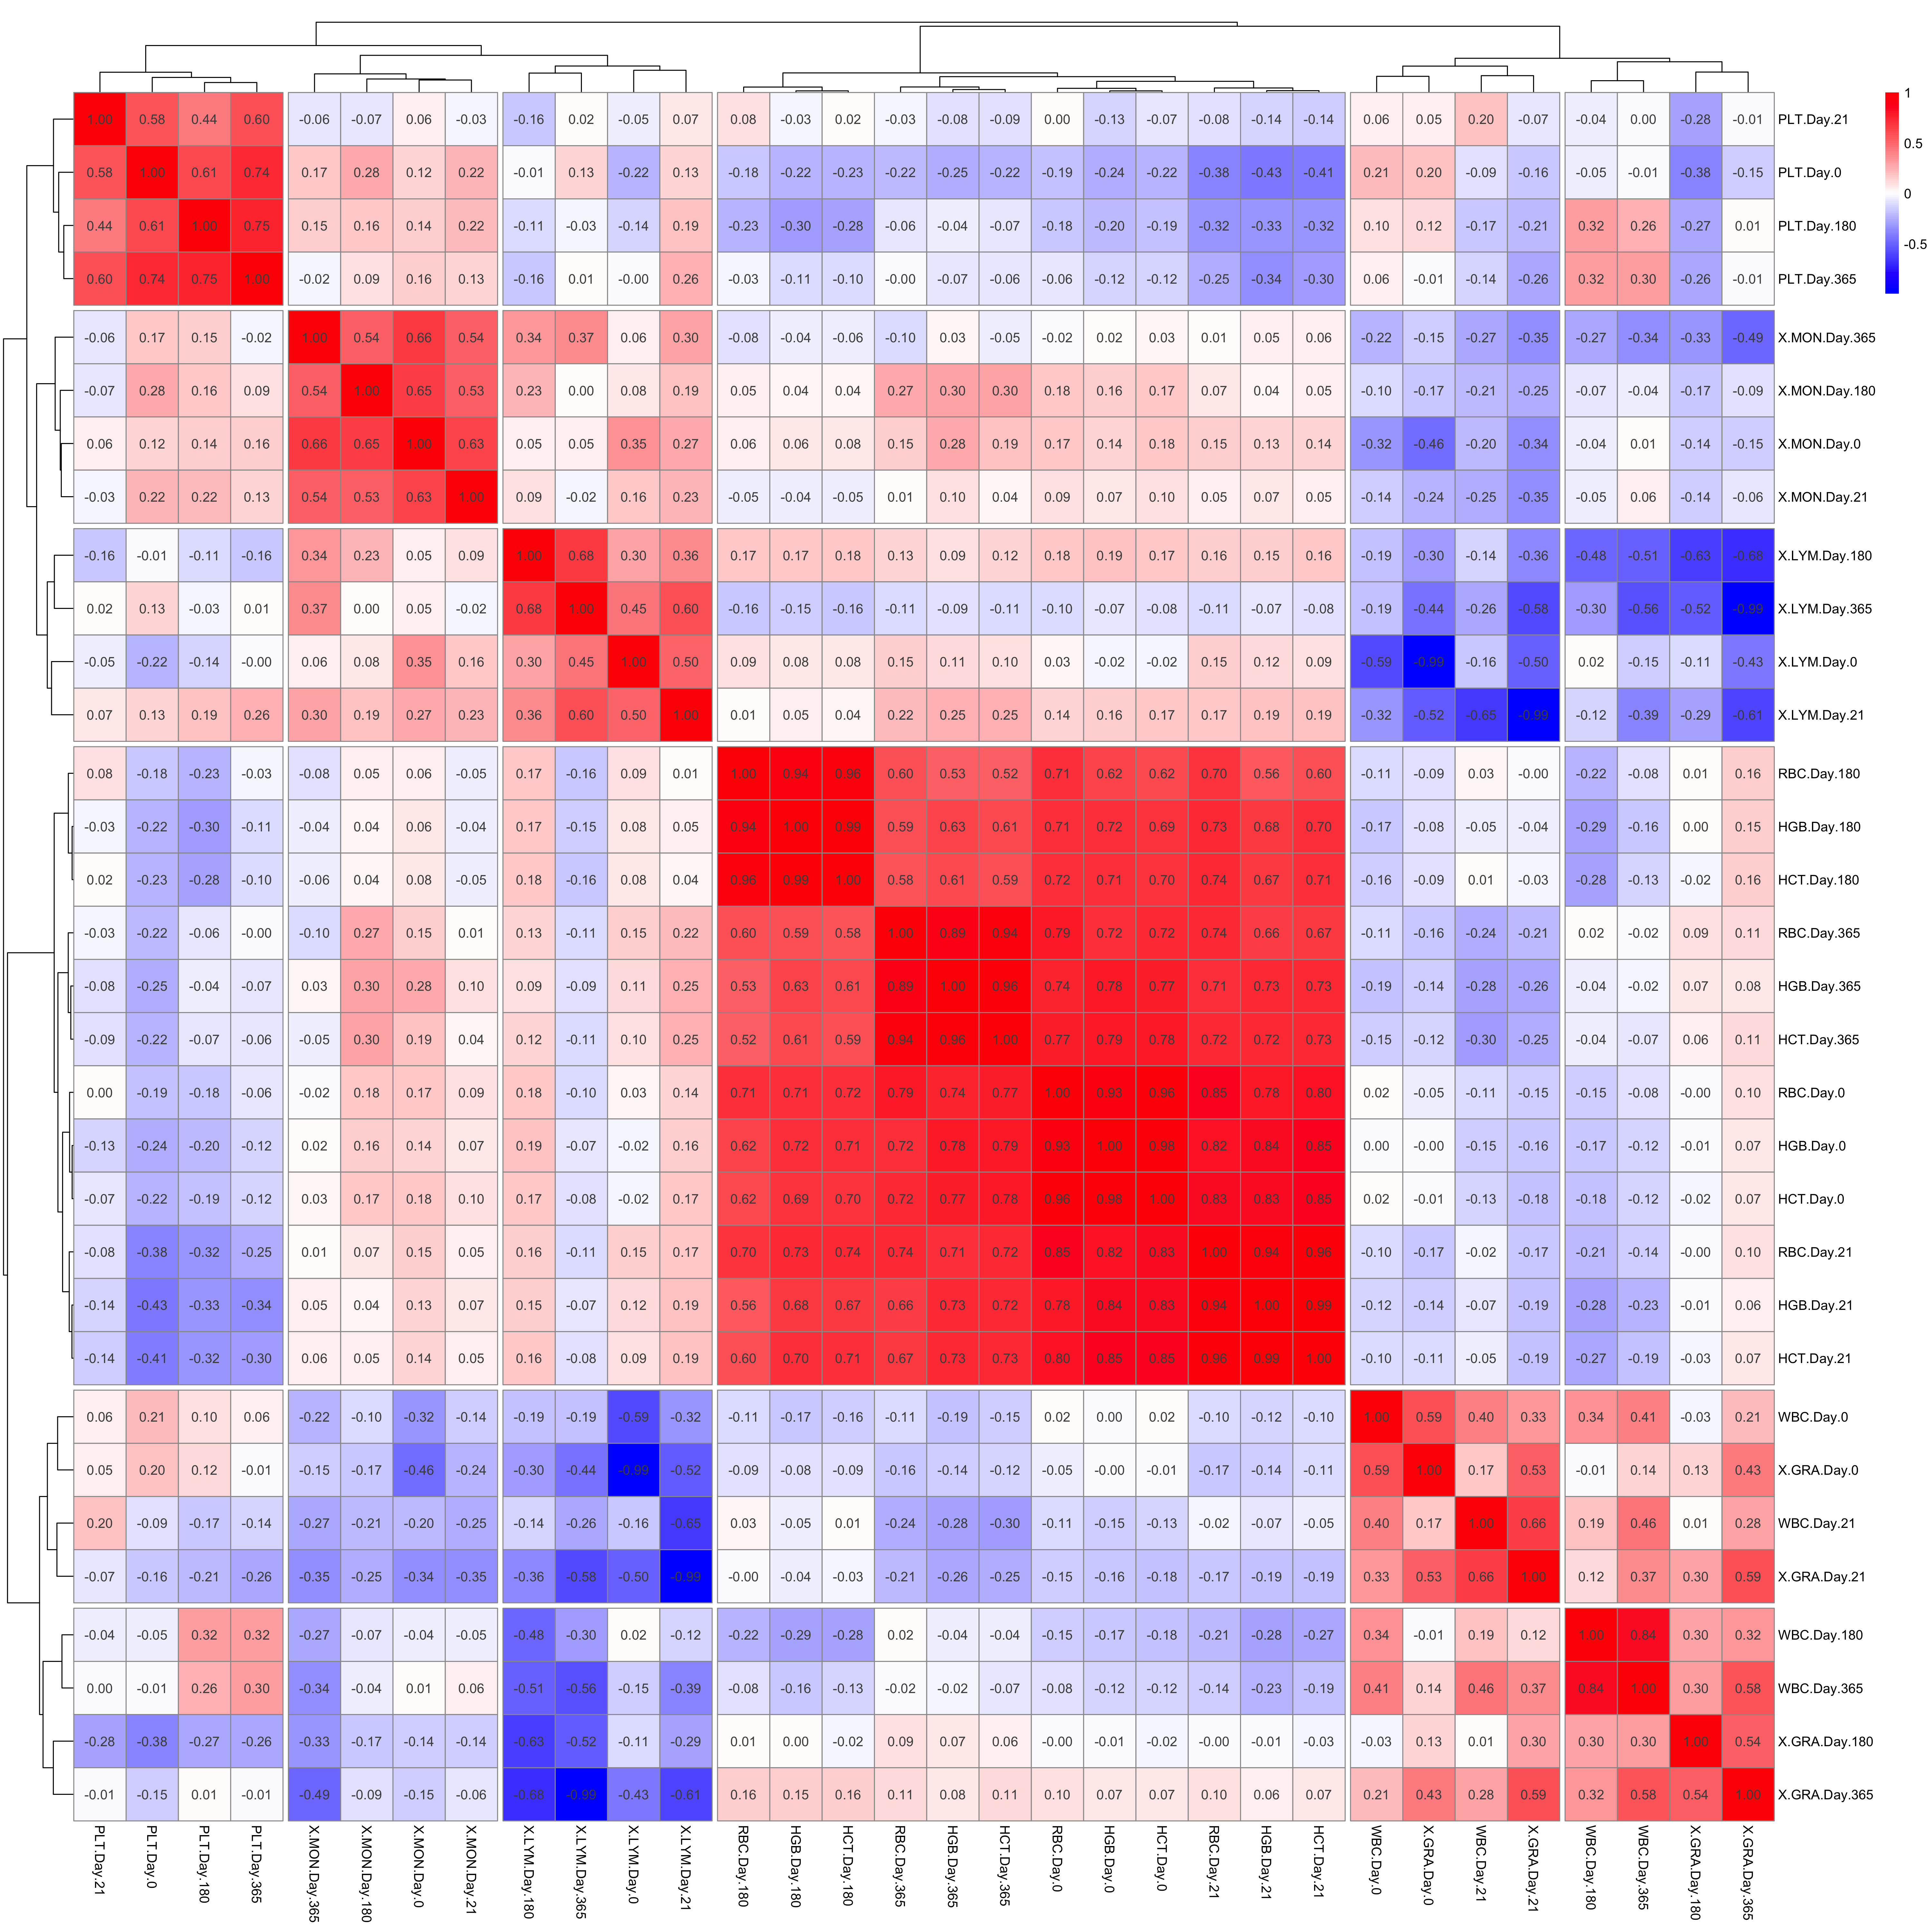
\includegraphics[width=0.8\textwidth]{images/Cytometry_euclidean_distance.png}
  \caption{Correlation heatmap of the cytometry data using Ward.D2 clustering.}
  \label{fig:cytometry_heatmap}
\end{figure}
\subsection{TCR Metrics}
\noindent

\begin{itemize}
  \item \textbf{Cluster 1: (RBC, HGB, HCT)} \\
  RBC (red blood cell count), HGB (hemoglobin), and HCT (hematocrit) are all interrelated measures of erythrocyte mass and oxygen-carrying capacity. Because they essentially quantify the same biological component—namely, red blood cells in circulation—their values often move in tandem. At Day~1, the heatmap reveals high correlation coefficients (e.g., 0.89--0.99) among RBC, HGB, and HCT, and similar correlation patterns emerge at Day~0, Day~21, Day~180, and Day~365, reinforcing their consistent co-variation over time. Ward.D2 naturally groups  these three parameters into a single cluster by minimizing within-cluster variance. Even when only Day~1 is considered, RBC, HGB, and HCT remain tightly linked, underscoring their close functional relationship.
\end{itemize}

\subsection{RNA Data}
\todo{...}\\

\section{Integrated Correlation Analysis}
\noindent
After analyzing each dataset separately, I combine them into two integrated datasets. The first integrated dataset merges the Cytokine and Cytometry data, while the second integrates Cytokine, Cytometry, and RNA data. The second combined dataset will be used in later stages of the thesis. This integrated analysis provides insights into how variables from different data types (e.g., cytokine levels, cell counts, and RNA expression) correlate with one another. Although this approach increases the number of correlations observed, it also introduces challenges such as higher dimensionality and potential confounding effects.\\
\\
\todo{...}\\

\bibliographystyle{plain}
\bibliography{references}

\end{document}
